\newpage%
\normalfont%
% \vskip -2\baselineskip plus -1fil%
\begin{IEEEbiography}[{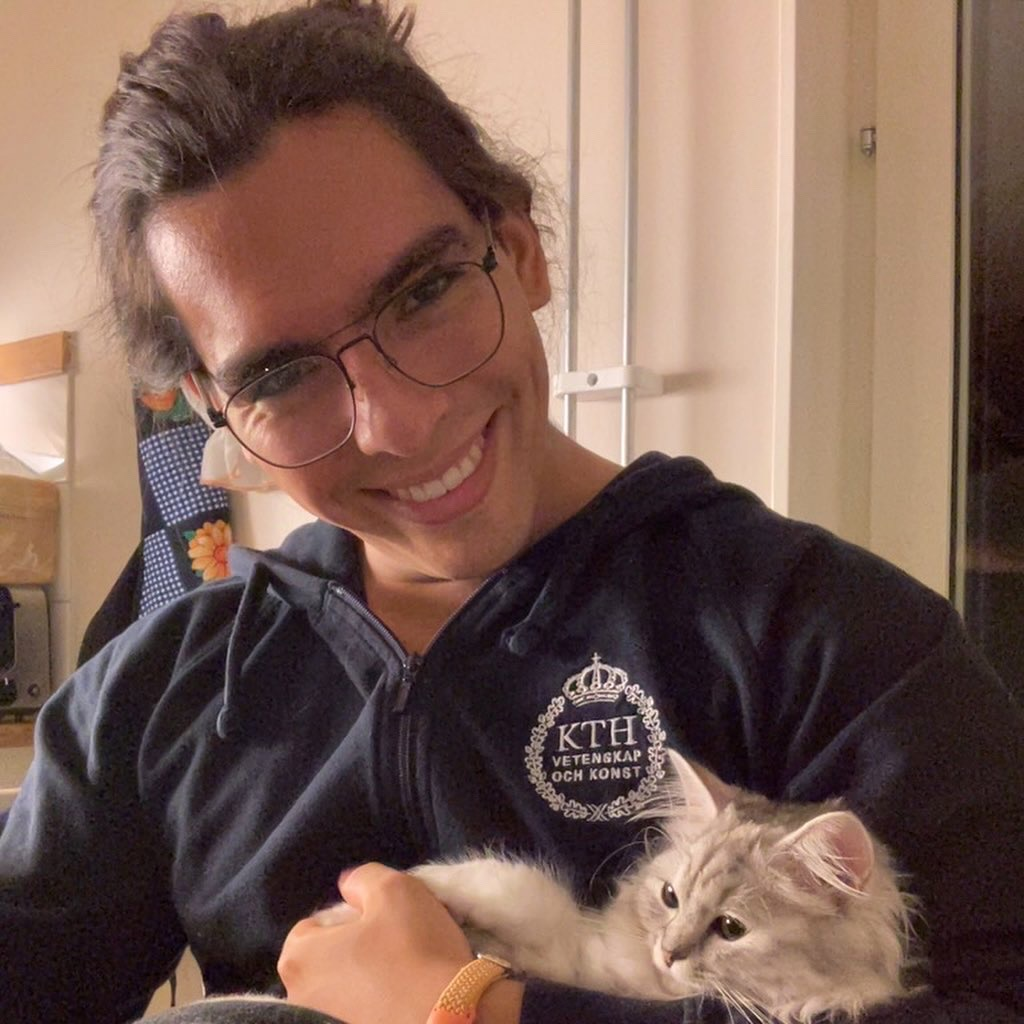
\includegraphics[width=1in,height=1.25in,clip,keepaspectratio]{bios/manuel.jpeg}}]%
    Manuel Olguín~Muñoz obtained in 2017 his B.Sc.Eng.\ in Computing and Engineer's Degree in Computing from Universidad de Chile.
    He is currently a final-year Ph.D. candidate at the division of Information Science and Engineering, School of Electrical Engineering and Computer Science (EECS), at KTH Royal Institute of Technology, Sweden.
    His research interests lie in the benchmarking and performance analysis of Edge Computing infrastructures and the applications deployed on them, in particular with respect to human-in-the-loop applications and cyber-physical systems.
    He also has an active role in designing and implementing the first 5G-enabled Edge Computing testbed at KTH and northern Europe.
\end{IEEEbiography}
% \vskip -2\baselineskip plus -1fil%
\begin{IEEEbiography}[{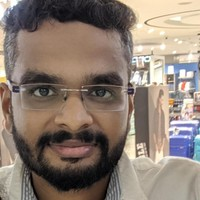
\includegraphics[width=1in,height=1.25in,clip,keepaspectratio]{bios/vishnu.jpeg}}]%
    Vishnu Narayanan Moothedath is a doctoral student in the department of Intelligent Systems under the School of Electrical Engineering and Computer Science (EECS) at KTH Royal Institute of Technology from 2021.
    He completed his master's degree in Communication Systems from the Indian Institute of Technology (IIT) Madras in 2016 and his bachelor's degree in Electrics and Communication Engineering from the National Institute of Technology (NIT) Calicut in 2012.
    He has also worked for five years in the cellular industry with Intel India Pvt.\ Ltd.\ and Apple India Pvt.\ Ltd.\ in their respective LTE/5G-NR base-band modem group.
    His current research is in the area of edge computing and performance optimization with a specific focus on improving the energy efficiency and responsiveness of edge computing systems through optimized sampling.
\end{IEEEbiography}
% \vskip -2\baselineskip plus -1fil%
\begin{IEEEbiography}[{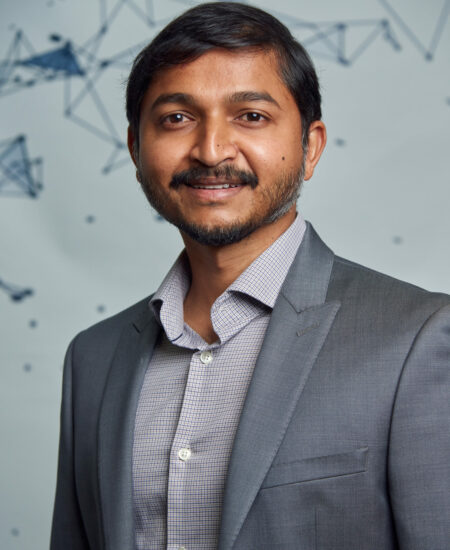
\includegraphics[width=1in,height=1.25in,clip,keepaspectratio]{bios/jaya.jpeg}}]%
    Jaya Prakash Champati (IEEE member) received his bachelor of technology degree from the National Institute of Technology Warangal, India in 2008, and master of technology degree from the Indian Institute of Technology (IIT) Bombay, India in 2010.
    He received his Ph.D. in Electrical and Computer Engineering from the University of Toronto, Canada in 2017.
    From 2017--2020, he was a post-doctoral researcher with the division of Information Science and Engineering, EECS, KTH Royal Institute of Technology,Sweden.
    He is currently a Research Assistant Professor at IMDEA Networks Institute, Madrid, Spain.
    His general research interest is in the design and analysis of algorithms for scheduling problems that arise in networking and information systems.
    Currently, his research focus is in Edge Computing/Intelligence, Age of Information, Cyber-Physical Systems (CPS), and Internet of Things (IoT).
    Prior to joining PhD he worked at Broadcom Communications, where he was involved in developing the LTE MAC layer.
    He was a recipient of the best paper award at IEEE National Conference on Communications, India, 2011.
\end{IEEEbiography}
% \vskip -2\baselineskip plus -1fil%
\begin{IEEEbiography}[{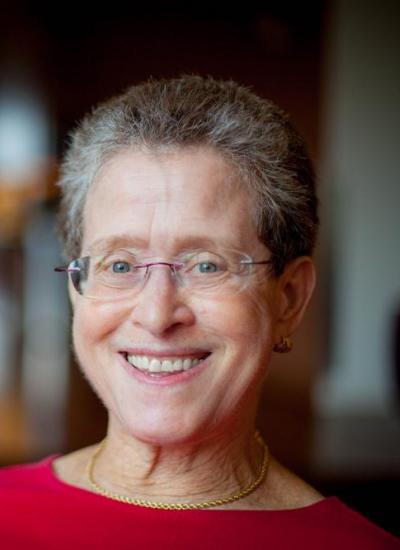
\includegraphics[width=1in,height=1.25in,clip,keepaspectratio]{bios/bobby.jpeg}}]%
    Roberta L. Klatzky (Fellow, IEEE) received the Ph.D. degree in cognitive psychology from Stanford University, Stanford, CA, USA.
    She is currently the Charles J. Queenan, Jr. University Professor with Carnegie Mellon University, Pittsburgh, PA, USA, where she is a Member of the Department of Psychology, Human-Computer Interaction Institute, and Neuroscience Institute.
    Her research interests include human perception and cognition, with special emphasis on spatial cognition and haptic perception.
\end{IEEEbiography}
% \vskip -2\baselineskip plus -1fil%
\begin{IEEEbiography}[{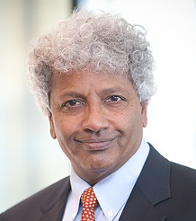
\includegraphics[width=1in,height=1.25in,clip,keepaspectratio]{bios/satya.jpeg}}]%
    Mahadev ``Satya'' Satyanarayanan's multi-decade research career has focused on the challenges of performance, scalability, availability and trust in information systems that reach from the cloud to the mobile edge of the Internet.
    In the course of this work, he has pioneered many advances in distributed systems, mobile computing, pervasive computing, and the Internet of Things (IoT).
    Most recently, his seminal 2009 publication ``The Case for VM-based Cloudlets in Mobile Computing'' and the ensuing research has  led to the emergence of Edge Computing (also known as ``Fog Computing'').
    Satya is the Carnegie Group Professor of Computer Science at Carnegie Mellon University.
    He received the Ph.D. in Computer Science from Carnegie Mellon, after Bachelor's and Master's degrees from the Indian Institute of Technology, Madras.
    He is a Fellow of the ACM and the IEEE.
\end{IEEEbiography}
\newpage%
% \vskip -2\baselineskip plus -1fil%
\begin{IEEEbiography}[{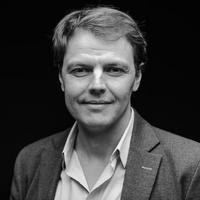
\includegraphics[width=1in,height=1.25in,clip,keepaspectratio]{bios/james.jpeg}}]%
    James Gross received his Ph.D. degree from TU Berlin in 2006.
    From 2008--2012 he was with RWTH Aachen University as assistant professor and research associate of RWTH's center of excellence on Ultra-high speed Mobile Information and Communication (UMIC).
    Since November 2012, he has been with the Electrical Engineering and Computer Science School, KTH Royal Institute of Technology, Stockholm, where he is professor for machine-to-machine communications.
    At KTH, James served as director for the ACCESS Linnaeus Centre from 2016 to 2019, while he is currently associate director in the newly formed KTH Digital Futures research center, as well as co-director in the newly formed VINNOVA competence center on Trustworthy Edge Computing Systems and Applications (TECoSA).
    His research interests are in the area of mobile systems and networks, with a focus on critical machine-to-machine communications, edge computing, resource allocation, as well as performance evaluation.
    He has authored over 150 (peer-reviewed) papers in international journals and conferences.
    His work has been awarded multiple times, including the best paper awards at ACM MSWiM 2015, IEEE WoWMoM 2009 and European Wireless 2009.
    In 2007, he was the recipient of the ITG/KuVS dissertation award for his Ph.D. thesis.
\end{IEEEbiography}